%You can leave alone everything before Line 79.
\documentclass{article}
\usepackage{url,amsfonts, amsmath, amssymb, amsthm,color, enumerate}
% Page layout
\setlength{\textheight}{8.75in}
\setlength{\columnsep}{2.0pc}
\setlength{\textwidth}{6.5in}
\setlength{\topmargin}{0in}
\setlength{\headheight}{0.0in}
\setlength{\headsep}{0.0in}
\setlength{\oddsidemargin}{0in}
\setlength{\evensidemargin}{0in}
\setlength{\parindent}{1pc}
\newcommand{\shortbar}{\begin{center}\rule{5ex}{0.1pt}\end{center}}
%\renewcommand{\baselinestretch}{1.1}
% Macros for course info
\newcommand{\courseNumber}{ME 552}
\newcommand{\courseTitle}{Mechatronics}
\newcommand{\semester}{Fall 2012}
\newcommand{\xxx}[1]{\textcolor{red}{#1}}
% Theorem-like structures are numbered within SECTION units
\theoremstyle{plain}
\newtheorem{theorem}{Theorem}[section]
\newtheorem{lemma}[theorem]{Lemma}
\newtheorem{corollary}[theorem]{Corollary}
\newtheorem{proposition}[theorem]{Proposition}
\newtheorem{statement}[theorem]{Statement}
\newtheorem{conjecture}[theorem]{Conjecture}
\newtheorem{fact}{Fact}
%definition style
\theoremstyle{definition}
\newtheorem{definition}[theorem]{Definition}
\newtheorem{example}{Example}
\newtheorem{problem}[theorem]{Problem}
\newtheorem{exercise}{Exercise}
\newtheorem{algorithm}{Algorithm}
%remark style
\theoremstyle{remark}
\newtheorem{remark}[theorem]{Remark}
\newtheorem{reduction}[theorem]{Reduction}
%\newtheorem{question}[theorem]{Question}
\newtheorem{question}{Question}
%\newtheorem{claim}[theorem]{Claim}
%
% Proof-making commands and environments
\newcommand{\beginproof}{\medskip\noindent{\bf Proof.~}}
\newcommand{\beginproofof}[1]{\medskip\noindent{\bf Proof of #1.~}}
\newcommand{\finishproof}{\hspace{0.2ex}\rule{1ex}{1ex}}
\def\therefore{\boldsymbol{\text{ }
\leavevmode
\lower0.4ex\hbox{$\cdot$}
\kern-.5em\raise0.7ex\hbox{$\cdot$}
\kern-0.55em\lower0.4ex\hbox{$\cdot$}
\thinspace\text{ }}}

\newenvironment{solution}[1]{\medskip\noindent{\bf Problem #1.~}}{\shortbar}

%====header======
\newcommand{\solutions}[4]{
%\renewcommand{\thetheorem}{{#2}.\arabic{theorem}}
\vspace{-2ex}
\begin{center}
{\small  \courseNumber, \courseTitle
\hfill {\Large \bf {#1} }\\
\semester, University of Michigan, Ann Arbor \hfill
{\em Date: #3}}\\
\vspace{-1ex}
\hrulefill\\
\vspace{4ex}
{\LARGE Lab Assignment #2}\\
\vspace{2ex}
\end{center}
\begin{trivlist}
\item \textsc{Team members:\\} {#4}
\end{trivlist}
\noindent
\shortbar
\vspace{3ex}
}
% math macros
\newcommand{\defeq}{\stackrel{\textrm{def}}{=}}
\newcommand{\Prob}{\textrm{Prob}}
%==
\usepackage{graphicx}
\usepackage{xfrac}
\usepackage{amsmath}
\begin{document}
%%%%%%%%%%%%%%%%%%%%%%%%%%%%%%%%%%%%%%%%%%%%%%%%%
%\solutions{Your name}{Problem Set Number}{Date of preparation}{Collaborators}{Prover}{Verifiers}
\solutions{}{2: MagLev}{\today}{Shiva Ghose, @gshiva\\ John Peterson, @jrpeters\\ Peter Turpel, @pturpel\\ Chan-Rong Lin, @pmelin}
%%%%%%%%%%%%%%%%%%%%%%%%%%%%%%%%%%%%%%%%%%%%%%%%%
%\renewcommand{\theproblem}{\arabic{problem}} 
%%%%%%%%%%%%%%%%%%%%%%%%%%%%%%%%%%%%%%%%%%%%%%%%%
%
% Begin the solution for each problem by
% \begin{solution}{Problem Number} and ends it with \end{solution}
%
% the solution for Problem 
\section*{Teamwork Participation Pledge :: Team 1}

I attest that I have made a fair and equitable contribution to this lab and submitted 
assignment. \\

My signature also indicates that I have followed the University of Michigan Honor Code, 
while working on this lab and assignment.\\

I accept my responsibility to look after all of the equipment assigned to me and my team, 
and that I have read and understood the X50 Lab Rules.\\

\begin{table}[h]
\begin{center}
    \begin{tabular}{|c|c|c|}
        \hline
        \textbf{Name} & \textbf{Email}     & \textbf{ \ \ \ \ \  \ \  \ \ \ \ \  \ \ Signature  \ \ \ \ \  \ \ \ \ \ \ \  \ \ } \\ \hline
        	~& ~& ~\\
	~& ~& ~\\
	Shiva Ghose   & gshiva@umich.edu   & ~                  \\
	~& ~& ~\\
	~& ~& ~\\ \hline 
	~& ~& ~\\
	~& ~& ~\\
        John Peterson & jrpeters@umich.edu & ~                  \\ 
	~& ~& ~\\
	~& ~& ~\\ \hline 
	~& ~& ~\\
	~& ~& ~\\
        Peter Turpel   & pturpel@umich.edu & ~                  \\
	~& ~& ~\\
	~& ~& ~\\ \hline 
	~& ~& ~\\
	~& ~& ~\\
        Chan-Rong Lin   & pmelin@umich.edu & ~                  \\
	~& ~& ~\\
	~& ~& ~\\ \hline 
        \hline
    \end{tabular}
\end{center}
\end{table}

\newpage
\begin{center}
\section*{Part B}
\end{center}
\section*{Question 1}

\subsection*{a.}

\subsubsection*{Break Beam Sensor}

\textbf{Assumptions} 
\begin{itemize}
\item Neglect the effects of diffraction.
\item Light rays are parallel. 
\item Neglect reflection of IR light by the polished ball stand.
\end{itemize}
As a consequence of the first two assumptions the IR beam from the LED to the photo-transistor can be modeled as a cylinder.  The shadow cast by the sphere is then simply a circle with radius equal to the radius of the sphere itself.  This also means that the distance between the sphere and the IR LED does not matter, instead the only values that matter are the radius of the IR beam, the radius of the sphere, and the perpendicular distance between the axis of the beam and the center of the sphere.  The amount of light received by the photo-transistor can then simply be modeled as the intersection of two circles in 2-dimensions as shown in figure \ref{Q1_a1}. \\

\[
  Radiance \hspace{0.1cm} Fraction = \left\{
  \begin{array}{l l}
    \frac{A_{beam} - A_{sphere}}{A_{beam}} & \quad \text{if } r_{sphere} + |d| < r_{beam} \\
    0 & \quad \text{if } r_{beam} + |d| < r_{sphere} \\
    1 & \quad \text{if } |d| < r_{beam} + r_{sphere} \\
    \frac{A_{beam} - A_{Overlap}}{A_{beam}} & \quad \text{if } |d| < r_{sphere} + r_{beam} \\
  \end{array} \right.
\]

\xxx{Format this part to look a bit nicer} \\
\textbf{Where:}
$$ A_{beam} = \pi r_{beam}^2, \hspace{1cm} A_{sphere} = \pi r_{sphere}^2 $$ 
$$ y = \frac{d^2+r_{beam}^2-r_{sphere}^2}{2d}, \hspace{1cm} d_{beam}=y, \hspace{1cm} d_{sphere}=d-y=\frac{d^2-r_{beam}^2+r_{sphere}^2}{2d} $$
$$ A_{Obeam} = r_{beam}^2 \cos^{-1} (\frac{d_{beam}}{r_{beam}})-d_{beam} \sqrt{r_{beam}^2-d_{beam}^2}$$ 
$$ A_{Osphere} = r_{sphere}^2 \cos^{-1} (\frac{d_{sphere}}{r_{sphere}})-d_{sphere} \sqrt{r_{sphere}^2-d_{sphere}^2}$$
$$ A_{Overlap} = A_{Obeam} + A_{Osphere} $$

\begin{figure}
\begin{center}
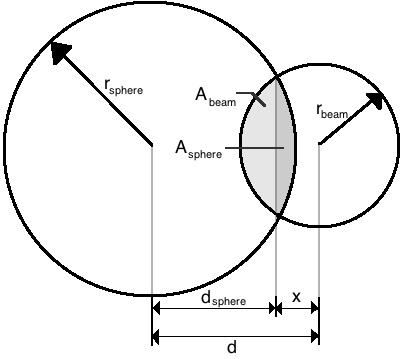
\includegraphics[width = 9cm]{beam_sphere_diagram.png}
\caption{Planar approximation of IR beam occluded by steel sphere}
\label{Q1_a1}
\end{center}
\end{figure}

\subsubsection*{Driver Circuit}
\textbf{Assumptions}
\begin{itemize}
\item Op-Amp Golden Rules: voltage at inverting and non-inverting terminals is equal and op-amp input impedance is infinite
\end{itemize}

The electromagnet driver is a simple op-amp circuit, shown in figure \ref{Q1_a2}, which is designed to pass a specific current through the electromagnet for a a given input voltage.  The voltage at the non-inverting input can be simply determined by applying the voltage divider rule.  The voltage at the inverting input is now known allowing us to apply Ohm's Law to determine the current through $R_{3}$ and therefore through the electromagnet.  Notice that the resistance of the electromagnet does not affect the current provided by the driver circuit.

$$ V^{+}=\frac{R_2}{R_1+R_2}V_{in} \hspace{1cm} I_{EM}=\frac{V^{+}}{R_3}=\frac{1}{R_3}\left(\frac{R_2}{R_1+R_2}\right)V_{in} = DV_{in}$$

\begin{figure}
\begin{center}
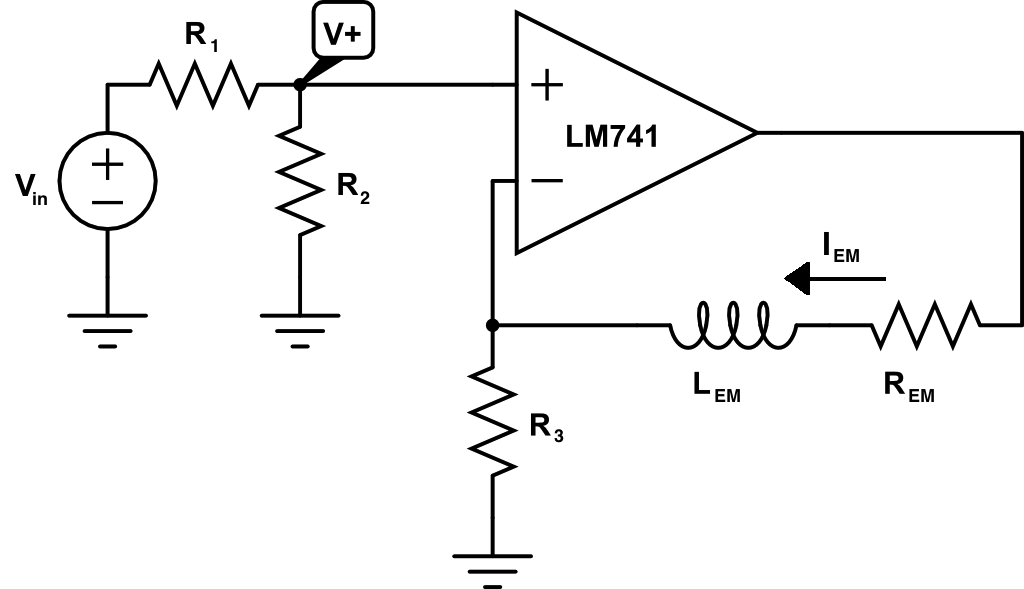
\includegraphics[width = 9cm]{em_driver_circuit.png}
\end{center}
\label{Q1_a2}
\caption{Electromagnet Driver Circuit}
\end{figure}

\subsubsection*{Electromagnet}
\textbf{Assumptions}

\begin{figure}[htb]
\begin{minipage}[b]{0.45\linewidth}
\centering
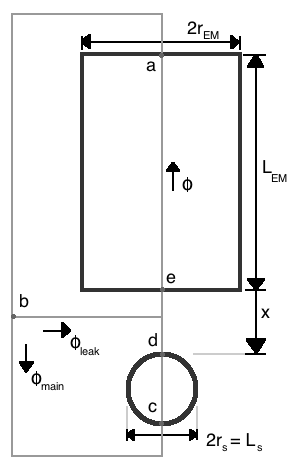
\includegraphics[width = 7cm]{flux_diagram.png}
\caption{Approximate Flux paths taken through our system}
\label{Q1_a3L}
\end{minipage}
\hspace{0.5cm}
\begin{minipage}[b]{0.45\linewidth}
\centering
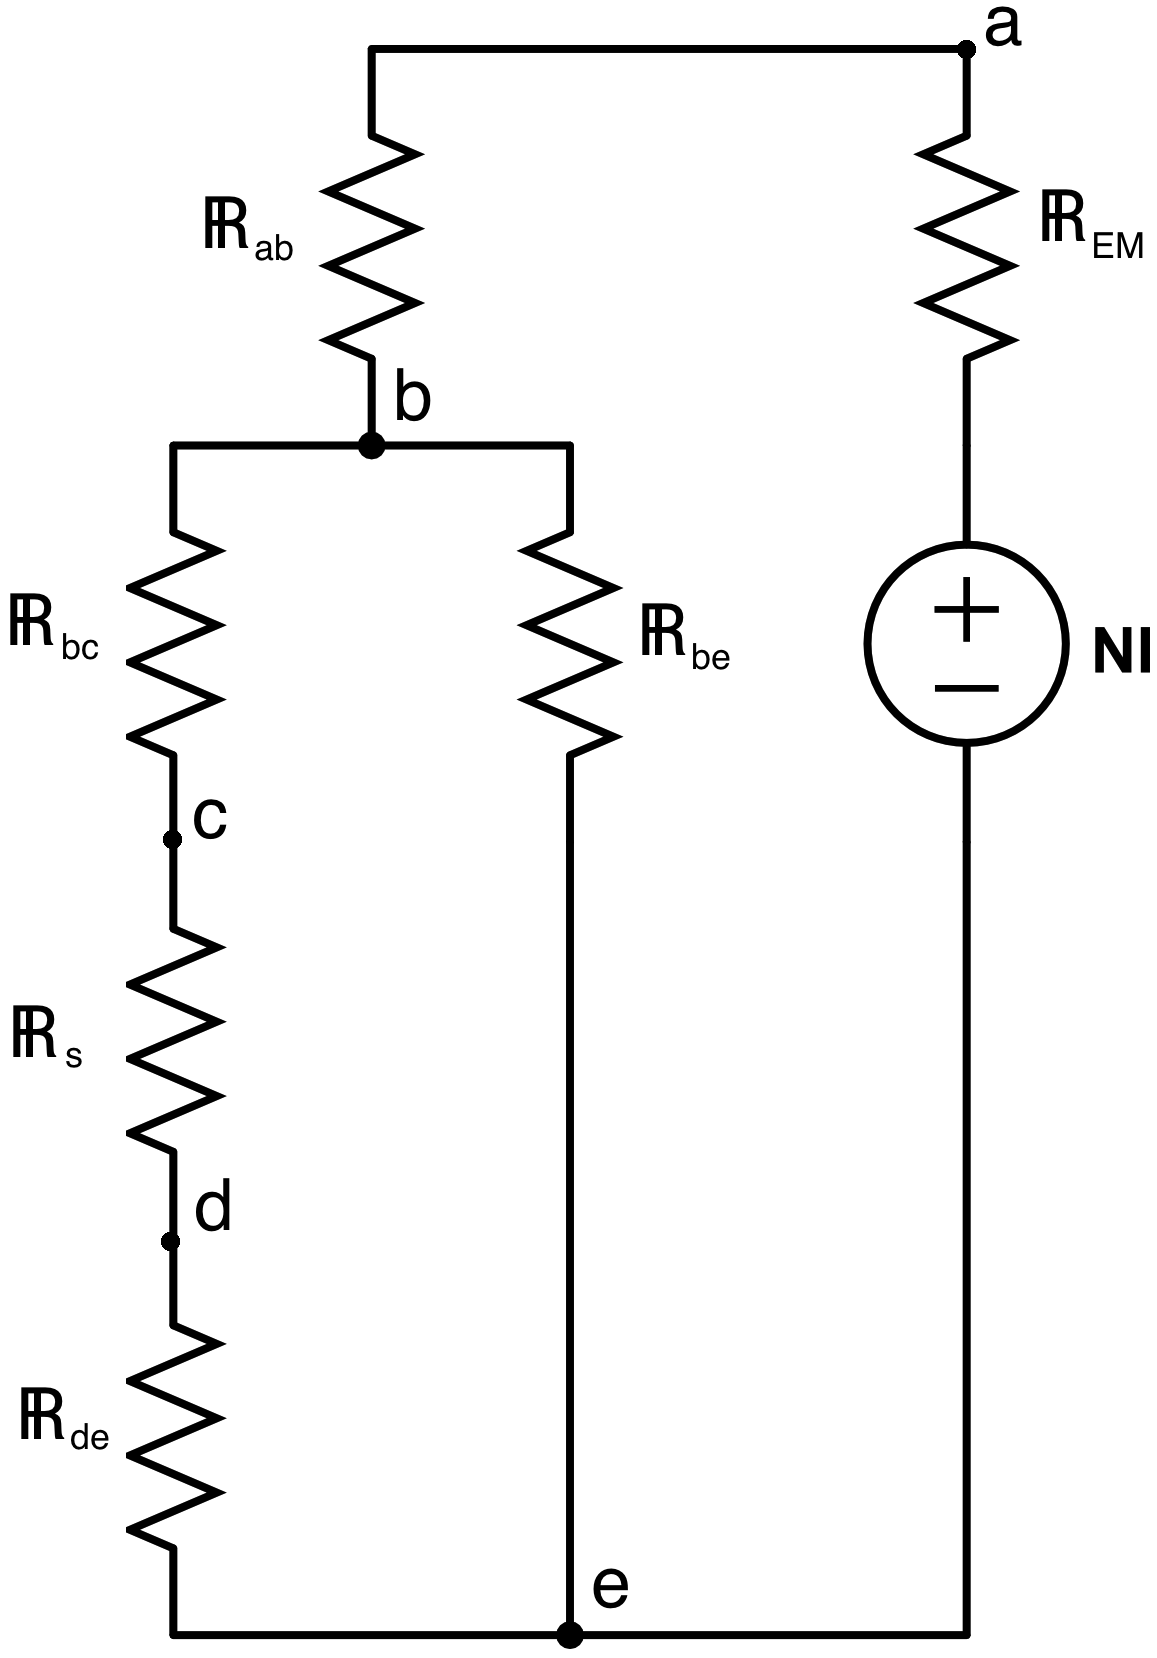
\includegraphics[width = 8cm]{magnetic_circuit.png}
\caption{Equivalent Magnetic Circuit}
\label{Q1_a3R}
\end{minipage}
\end{figure}

\begin{itemize}
\item $ \mu_{Al} \approx \mu_{Cu} \approx \mu_{air} $ , where $\mu_x$ is the absolute permeability of material $x$
\item $ \mu_{steel} \gg \mu_{air} $
\item We can model the steel sphere as a cylinder with its axis collinear with the electromagnet  \\ 
$$A_{cd} \approx A_{s} = \pi * r_{sphere}^2 $$ 
\item We can neglect the effects of fringing on the cross-sectional area and assume particular dimensions of area of paths through the air that are consistent with the solid objects in the system \\
$$ A_{EM} = \pi*r_{EM}^2 \approx A_{ab} \hspace{1cm} A_{s} \approx A_{bc} \approx A_{de} \hspace{1cm} A_{EM} \approx A_{be} + A_{bc} $$ 
\item Path length from b to c (see figure \ref{Q1_a2}) does not vary with x: 
$ \frac{\partial}{\partial x} (L_{bc}) = 0$
\item The sphere remains in line with the axis of the electro magnet and $ x > 0$
\end{itemize}

Drawing out approximate flux paths yields the following diagram in figure \ref{Q1_a3L} which can be converted to the following magnetic circuit , shown in figure \ref{Q1_a3R}, by applying Ampere's Law and Maxwell's $2^{nd}$ law which yield the following three equations. 

$$ NI = \phi \left (\mathbb{R}_{EM} + \mathbb{R}_{ab}\right) + \phi_{main} \left( \mathbb{R}_{bc}+\mathbb{R}_{s}+\mathbb{R}_{dc} \right) $$
$$ NI = \phi \left( \mathbb{R}_{EM} + \mathbb{R}_{ab} \right) + \phi_{leak} \left( \mathbb{R}_{be} \right) $$
$$ \phi = \phi_{main} + \phi_{leak} $$


$$ \mathbb{R}_{EM} = \frac{L_{EM}}{A_{EM}\mu_{air}}  \hspace{1cm} \mathbb{R}_{ab} = \frac{L_{ab}}{A_{EM}\mu_{air}} \hspace{1cm} \mathbb{R}_{bc} = \frac{L_{bc}}{(A_{s})\mu_{air}} \hspace{1cm} \mathbb{R}_{de} = \frac{x}{A_{A_{s}}\mu_{air}} \hspace{1cm} $$ $$ \mathbb{R}_{be} = \frac{L_{be}}{(A_{EM} - A_{s})\mu_{air}}  \hspace{1cm}  \mathbb{R}_{s} = \frac{2*r_{sphere}}{A_{s}\mu_{steel}} \approx 0$$

Solving the $2^{nd}$ equation for $\phi_{leak}$ gives:

$$\phi_{leak} = C_{0}\left( NI-C_{1}\phi_{main} \right)$$ 
$$C_{0} = \frac{\mu_{air} A_{EM} (A_{EM} - A_{s})}{L_{be} A_{EM} + (L_{EM} + L_{ab})(A_{EM} - A_{s}))} \hspace{1cm} 
C_{1} = \frac{L_{EM} + L_{ab}}{\mu_{air} A_{EM}} $$

Substituting back into the $1^{st}$ equation lets us solve for $\phi_{main}$ yielding: 

$$ \phi_{main} = \frac{NI(1-C_{0}C_{1})}{C_{1} - C_{0} C_{1}^2 + \frac{L_{bc}}{\mu_{air} A_{s}} + \frac{x}{\mu_{air} A_{s}}} $$

With equations for our fluxes we can now compute the self inductance and from that compute the force exerted on the steel sphere as a function of position and current.

$$ \lambda = N \phi = L(x) I $$
$$ W(i,x) = (\sfrac{1}{2}) L(x) I^2 = (\sfrac{1}{2}) N \phi(x) I =(\sfrac{1}{2}) N I (\phi_{main}(x) + \phi_{leak}(x))$$
$$ F(i,x) = \frac{d}{dx} (W(i,x) )= (\sfrac{1}{2}) N I ( \frac{d}{dx} (\phi_{main}) + \frac{d}{dx} (\phi_{leak})) $$

$$ \frac{d}{dx}(\phi_{main}) = - \frac{N I (1 - C_{0}C_{1} \mu_{air} A_{s}}{(\mu_{air} A_{s}(C_{1} - C_{0} C_{1}^2 + C_{2}) + x)^2} dx$$

$$ \frac{d}{dx}(\phi_{leak}) = -C_{0} C_{1} \frac{d}{dx}(\phi_{main})$$

Putting this pair of terms together yields our final expression for the force.

$$ F_{EM}(x) = -\frac{1}{2} \left( 1 - C_{0}C_{1} \right)^2 \frac{\mu_{air} A_{s} N^2 }{(\mu_{air} A_{s}(C_{1} - C_{0} C_{1}^2 + C_{2}) + x)^2} I^2 $$

We can then condense these terms to arrive at a simple equation to model the force, shown below.  Where values for A and B can be obtained experimentally.

$$ F_{EM}(x) = -\frac{A I^2}{(B+x)^2} $$

\subsubsection*{Steel Sphere \& Magnet System}
\textbf{Assumptions}
\begin{itemize}
\item Air resistance is negligible.
\item The steel sphere does not collide with the magnet: $x > 0$
\end{itemize}

According to Newton's second law the sum of the forces on an object is proportional to the acceleration of the object.  After constructing a free body diagram of our system shown in figure \ref{Q1_a4} we can very easily derive a model of the motion of our system.

$$ \sum F_x = mg + F_{EM} = mg -\frac{A I^2}{(B+x)^2} = m  \ddot{x}$$

\begin{figure}
\begin{center}
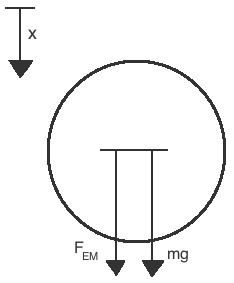
\includegraphics[width = 5cm]{freebodydiagram.png}
\label{Q1_a4}
\caption{Free body diagram of steel sphere.  Note: The x axis points downwards and our force was computed according to this convention, which is why their is a negative sign in the expression of the force generated by the electromagnet.}
\end{center}
\end{figure}

\subsection*{b.}
\subsubsection*{Break Beam Sensor}
The position sensor is very nearly linear with saturations at 0 and the full scale range.  The numerical derivative is easily obtained and useful in this case as the function is smooth, but the symbolic computation of the derivative, shown below, is far more involved. 

$$ d = x + 4.12 \hspace{1cm} \partial x=\partial d $$
$$ y = \frac{d^2+r_{beam}^2-r_{sphere}^2}{2d}=\frac{d}{2} + \frac{r_{beam}^2}{2d} - \frac{r_{sphere}^2}{2d} \hspace{1cm} \frac{\partial}{\partial d} y = \left(\frac{1}{2}  -\frac{r_{beam}^2}{2d^2} + \frac{r_{sphere}^2}{2d^2}\right) \partial d $$
$$ d_{beam}=y \hspace{1cm} \frac{\partial}{\partial d} d_{beam} =  \frac{\partial}{\partial d} y = \left(\frac{1}{2}  -\frac{r_{beam}^2}{2d^2} + \frac{r_{sphere}^2}{2d^2}\right) \partial d $$
$$  d_{sphere}=d-y \hspace{1cm}   \frac{\partial}{\partial d} d_{sphere} = 1\partial d - \frac{\partial}{\partial d} y = \left(1 - \frac{1}{2}  +\frac{r_{beam}^2}{2d^2} - \frac{r_{sphere}^2}{2d^2}\right) \partial d = \left(\frac{1}{2}  +\frac{r_{beam}^2}{2d^2} - \frac{r_{sphere}^2}{2d^2}\right) \partial d$$
$$ A_{Obeam} = r_{beam}^2 \cos^{-1} (\frac{d_{beam}}{r_{beam}})-d_{beam} \sqrt{r_{beam}^2-d_{beam}^2}$$ 

$$ \frac{\partial}{\partial d} A_{Obeam} = \left( -\frac{r_{beam}}{\sqrt{1 - \left(\frac{d_{beam}}{r_{beam}}\right)^2}} - \left( r_{beam}^2 - d_{beam}^2\right)^{\sfrac{1}{2}} + d_{beam}^2 \left( r_{beam}^2 - d_{beam}^2\right)^{\sfrac{-1}{2}} \right) \frac{\partial d_{beam}}{\partial d}$$

$$ A_{Osphere} = r_{sphere}^2 \cos^{-1} (\frac{d_{sphere}}{r_{sphere}})-d_{sphere} \sqrt{r_{sphere}^2-d_{sphere}^2} $$

$$ \frac{\partial}{\partial d} A_{Osphere} = \left( -\frac{r_{sphere}}{\sqrt{1 - \left(\frac{d_{sphere}}{r_{sphere}}\right)^2}} - \left( r_{sphere}^2 - d_{sphere}^2\right)^{\sfrac{1}{2}} + d_{sphere}^2 \left( r_{sphere}^2 - d_{sphere}^2\right)^{\sfrac{-1}{2}} \right) \frac{\partial d_{sphere}}{\partial d}$$

$$ A_{Overlap} = A_{Obeam} + A_{Osphere} \hspace{1cm}  \frac{\partial}{\partial d} A_{Overlap} = \frac{\partial}{\partial d} A_{Obeam} + \frac{\partial}{\partial d} A_{Osphere} $$

The set point we are linearizing about is in the area where the function above is well behaved:

$$ Radiance \hspace{0.1cm} Fraction = \frac{A_{beam} - A_{Overlap}}{A_{beam}} = 1 - \frac{A_{Overlap}}{A_{beam}} \hspace{1cm} $$

$$ \frac{\partial}{\partial d} \left( Radiance \hspace{0.1cm} Fraction \right) = \frac{1}{A_{beam}} \left( \frac{\partial}{\partial d} A_{Overlap} \right) $$

Taylor expansion allows us to approximate the Radiance Fraction about a certain distance $d_0$ as:

$$ Radiance \hspace{0.1cm} Fraction = R(d) = R(d_{0}) + \left. \frac{\partial \, R(d)}{\partial d} \right|_{d_{0}} \left( d - d_{0} \right) + \left. \frac{1}{2!} \frac{\partial^2 \, R(d)}{\partial d^2} \right|_{d_{0}} \left(d-d_{0}\right)^2 + ... $$

Dropping the higher order terms leaves us with a linear expression for the Radiance Fraction about a certain distance.

$$ R(d) \approx R(d_{0}) + \left. \frac{\partial \, R(d)}{\partial d} \right|_{d_{0}} \left( d - d_{0} \right) $$

Substituting our expression for d in terms of x yields:

$$ R(x) \approx R(x_{0} + 4.12) + \left. \frac{\partial \, R(x)}{\partial x} \right|_{x_{0}+4.12} \left( x - x_{0} \right) $$

Substituting our previous expressions in to obtain a single symbolic linear expression for the Radiance Fraction in terms of $x$, $r_{beam}$ and $r_{sphere}$ is possible but not particularly practical.  The appendix includes matlab code for computing $R'(d_{0})$.


%$$ R(d) \approx \left(1 - \frac{A_{Overlap}(d_{0})}{A_{beam}} \right) + \frac{1}{A_{beam}} \left( \frac{\partial}{\partial d} A_{Overlap}(d_{0}) \right) \left(d - d_{0} \right)$$
%
%$$ R(d) \approx \left(1 - \frac{1}{A_{beam}}\left(A_{Obeam}(d_{0}) + A_{Osphere}(d_{0}) \right) \right) + \frac{1}{A_{beam}} \left( \frac{\partial}{\partial d} A_{Obeam}(d_{0}) + \frac{\partial}{\partial d} A_{Osphere}(d_{0}) \right) \left(d - d_{0} \right)$$
%
%\begin{multline}
%R(d) \approx \left(1 - \frac{1}{A_{beam}}\left(r_{beam}^2 \cos^{-1} (\frac{d_{beam}}{r_{beam}})-d_{beam} \sqrt{r_{beam}^2-d_{beam}^2} \right. \right. \\ \left. \left.+ r_{sphere}^2 \cos^{-1} (\frac{d_{sphere}}{r_{sphere}})-d_{sphere} \sqrt{r_{sphere}^2-d_{sphere}^2} \right) \right) \\ + \frac{1}{A_{beam}} \left( \left( -\frac{r_{beam}^2}{\sqrt{1 - \left(\frac{d_{beam}}{r_{beam}}\right)^2}} - \left( r_{beam}^2 - d_{beam}^2\right)^{\sfrac{1}{2}} - d_{beam}^2 \left( r_{beam}^2 - d_{beam}^2\right)^{\sfrac{1}{2}} \right) \frac{\partial d_{beam}}{\partial d} \right. \\ \left. +  \left( -\frac{r_{sphere}^2}{\sqrt{1 - \left(\frac{d_{sphere}}{r_{sphere}}\right)^2}} - \left( r_{sphere}^2 - d_{sphere}^2\right)^{\sfrac{1}{2}} - d_{sphere}^2 \left( r_{sphere}^2 - d_{sphere}^2\right)^{\sfrac{1}{2}} \right) \frac{\partial d_{sphere}}{\partial d} \right) \left(d - d_{0} \right)
%\end{multline}
%
%\begin{multline}
%R(d) \approx \left(1 - \frac{1}{A_{beam}}\left(r_{beam}^2 \cos^{-1} (\frac{d_{beam}}{r_{beam}})-d_{beam} \sqrt{r_{beam}^2-d_{beam}^2} \right. \right. \\ \left. \left.+ r_{sphere}^2 \cos^{-1} (\frac{d_{sphere}}{r_{sphere}})-d_{sphere} \sqrt{r_{sphere}^2-d_{sphere}^2} \right) \right) \\ + \frac{1}{A_{beam}} \left( \left( -\frac{r_{beam}^2}{\sqrt{1 - \left(\frac{d_{beam}}{r_{beam}}\right)^2}} - \left( r_{beam}^2 - d_{beam}^2\right)^{\sfrac{1}{2}} - d_{beam}^2 \left( r_{beam}^2 - d_{beam}^2\right)^{\sfrac{1}{2}} \right) \frac{\partial d_{beam}}{\partial d} \right. \\ \left. +  \left( -\frac{r_{sphere}^2}{\sqrt{1 - \left(\frac{d_{sphere}}{r_{sphere}}\right)^2}} - \left( r_{sphere}^2 - d_{sphere}^2\right)^{\sfrac{1}{2}} - d_{sphere}^2 \left( r_{sphere}^2 - d_{sphere}^2\right)^{\sfrac{1}{2}} \right) \frac{\partial d_{sphere}}{\partial d} \right) \left(d - d_{0} \right)
%\end{multline}

\subsubsection*{Electromagnet \& Steel Sphere}
We can model the dynamic forces of attraction between the ball and the magnet as follows:
\xxx{shiva linearization goes here}

\xxx{still need overall linear mathematical model of the system}
\subsection*{c.}
The sensor has a non-linear relationship between ball position and output voltage.  The primary non-linearity in this system are the two saturations, at zero volts and the full scale value of 10 volts.  The central region is non-linear, but a linear function in this region provides a good approximation of the function.  Linear Controls theory may only be strictly applied to linear systems, because the Laplace Transform assumes linear time invariant systems.  Because of this assumption we must linearize our sensor about some nominal position.  The whole notion of a transfer function does not apply to a non-linear system so attempting to apply Linear Controls without the linearizion would be an oversight at best, if the system is pretty close to linear, or a complete disaster if it is not.  This non-linearity will cause the actual closed loop response to deviate from the results we would expect given the systems transfer function as we deviate from the nominal position.

\subsection*{d. Parameter Identification}

\subsubsection*{Break Beam Sensor}
To acquire data to measure the relationship between the displacement between the optical axis of the phototransistor and the steel sphere we sat the sphere on top of the stand and changed the height of the sphere stand and the magnet stand by known amounts recording the voltage from the phototransistor at each displacement value.  Theoretically we would expect the beam radius to be very close to the radius of the phototransistor while we would expect the blocking radius to be very close to the radius of the sphere.  Non-linear optimization of the non-linear model revealed that that the actual values, shown in table \ref{Q1_dt2} were reasonably close to our expected values.  The curve resulting from this fit and our data are shown in figure \ref{Q1_d1}.

\xxx{make sure table reference works!}

\begin{table}
\begin{center}
    \begin{tabular}{|c|c|c|}
        \hline
        ~      & Expected Radii (mm) & Fit Radii (mm) \\ \hline
        Rbeam  & 2.3650              & 1.398935       \\ 
        Rblock & 6.350               & 6.070821       \\
        \hline
    \end{tabular}
\end{center}
\label{Q1_dt2}
\caption{Expected and Fit values for beam radius and blocking radius}
\end{table}

\begin{figure}
\begin{center}
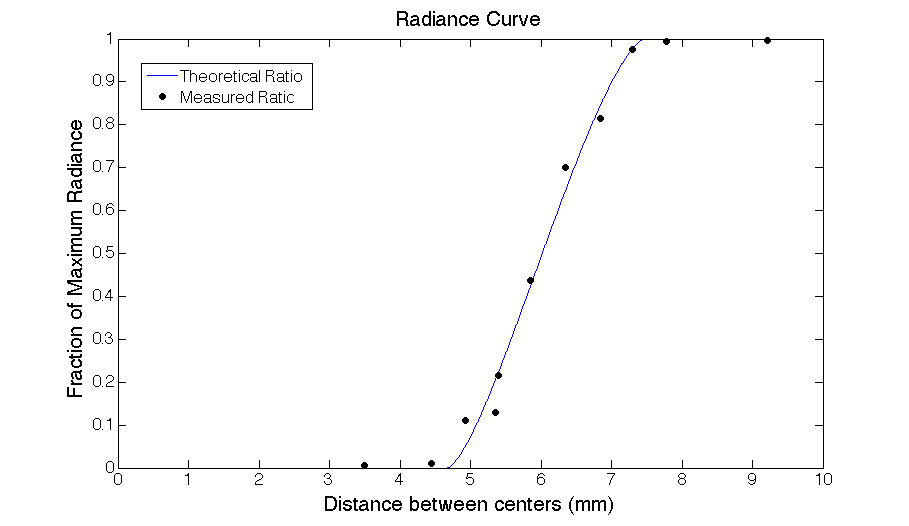
\includegraphics[width = 15cm]{SensorRadianceCurve.png}
\end{center}
\caption{Normalized Sensor Voltage Output vs distance from the optical axis}
\label{Q1_d1}
\end{figure}

There is a fixed offset between the displacement, measured from the optical axis of the phototransistor to the center of the sphere, used in figure \ref{Q1_d1}, from the x, measured from the bottom of the magnet to the top of the sphere, used in our controller.  This relationship can be obtained by examining the physical dimensions of the system, noted in table \ref{Q1_dt2} yielding the following expression for x in terms of d.

$$ x = \Delta + h_{magnet} - h_{s stand} - r_{s} \hspace{1cm} \Delta = d + h_{s stand} - h_{sensor} $$

Evaluating this equation and solving for $x$ yields the following relationship:

$$ x = d - 4.12 \text{ mm} $$

\begin{table}
\begin{center}
    \begin{tabular}{|c|c|}
        \hline
        ~                                    & Dimension (mm) \\ \hline
        Magnet Height $(h_{magnet}) $          & 130.73         \\ 
        Sphere on Stand Height $(h_{s stand})$ & 121.5          \\ 
        Sensor Height $(h_{sensor})$           & 128.5          \\ 
        Sphere Radius $(r_{s})$                & 6.35           \\
        \hline
    \end{tabular}
\end{center}
\caption{Physical Dimensions of the System}
\label{Q1_dt2}
\end{table}

\subsubsection*{Driver Circuit}

Theoretically the conversion from voltage to current for this system should be very straight forwards.  We used a multi-meter to measure the resistances, noted in table \ref{Q1_dt1}, and then plugged these values into our model yielding the following relationship between current and input voltage.

$$ I_{EM Expected}=\frac{1}{R_3}\left(\frac{R_2}{R_1+R_2}\right)V_{in} = \frac{1}{0.5 \,\Omega}\left(\frac{999 \,\Omega}{42.3 \,k\Omega + 999 \,\Omega}\right)V_{in} = 0.04233 \, V_{in}$$

However examining the actual current and voltage relationship obtained by using the current measuring functionality of the multi-meter revealed that the above relationship did not hold.  Our observations showed a steady state current even when the input voltage was 0, so we fit a general linear model to the data excluding the input voltages above the current saturation.  It is also worth noting that we expected the electromagnet current to saturate at 510 mA rather than the 400 mA seen here.

$$ I_{EM Fit} = D \, V_{in} + C = 0.1781 \, V_{in} - 0.0179  \quad \textbf{if } V_{in} \leq 2.3 \, V $$

\begin{figure}
\begin{center}
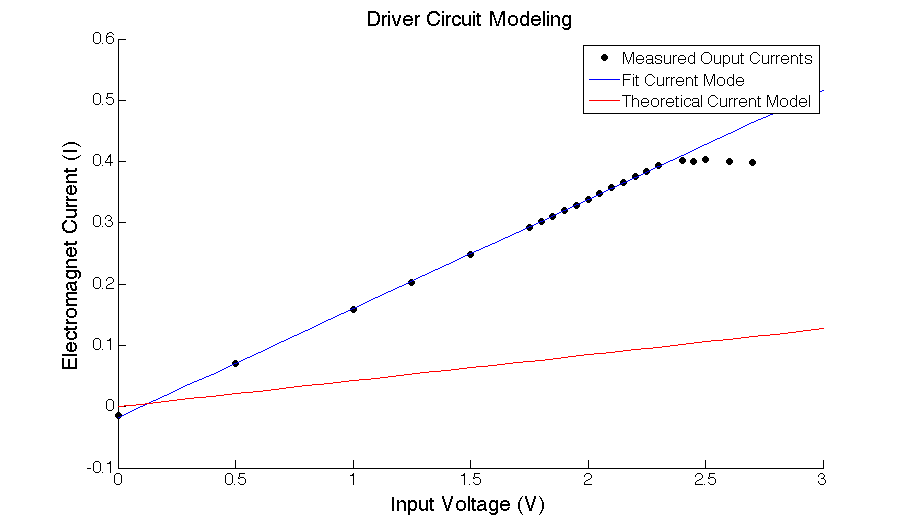
\includegraphics[width = 13cm]{DriverCircuitModel.png}
\end{center}
\label{Q1_d2}
\caption{Comparison of actual voltage current relationship with the fit model and the theoretical model}
\end{figure}

\begin{table}
\begin{center}
    \begin{tabular}{|c|c|}
        \hline
        Component & Resistance ($\Omega$) \\ \hline
        $R_{1}$   & 46200                 \\ 
        $R_{2}$   & 999                   \\ 
        $R_{3}$   & 0.5                   \\
        \hline
    \end{tabular}
\end{center}
\caption{Measured Resistances in driver circuit.}
\label{Q1_dt1}
\end{table}

\subsubsection*{Electromagnet}
Examining our model for the force exerted by the electromagnet we see that we have two unknowns, A and B.  Now that we have a working system we were able to conduct an experiment where we measured the amount of voltage sent to the driver to lift the steel sphere from a particular height.  We then attempted to perform non-linear optimization to determine A and B from this data however this computation diverged due to poor initial guesses for A and B.  To determine better initial guesses we symbolically solved for A and B as a function of two of these data points and then used these values as our initial estimate.  

$$ F(I,x) = \frac{A I^2}{(B+x)^2} $$
At equilibrium we know that the force exerted by the electromagnet must balance out the force of gravity on the sphere, this yields the following two expressions.
$$ mg = f = \frac{A I_{1}^2}{(B+x_{1})^2}  = \frac{A I_{2}^2}{(B+x_{2})^2} $$ 

We can solve the first expression for A.
$$ A = \frac{F (B + x_{1})^2}{I_{1}^2}$$

Then substituting the previous expression for A back into the $2^{nd}$ equation yields the following expression for B:
$$ B^2(1-R) + (2x_2-2x_1R)+x_2^2-x_1^2R = 0 \hspace{1cm} R = \frac{I_2^2}{I_1^1} $$

\xxx{why are their two solutions? what is the physical reason, and which one makes sense as the right one}

Choosing two of our x, I pairs allowed us to solve for plausible values of A and B which we used as initial guesses for the optimization allowing it to converge to the correct result.  It is important to note the difference between the two different fits presented in figure \ref{Q1_d3}.  Both are the result of non-linear regression to solve for our unknown parameters A and B.  However the errors that each minimize is different.  The Current fit, minimizes the expected amount of current draw at each of our measured x values from the actual amount of current drawn by the electromagnet.  The Force fit minimizes the error between the expected amount of force, computed for each pair of observed current and position, and the actual amount of force required to lift the steel sphere.  The fit error described in table \ref{Q1_dt2} refers to the error in each fits respective space.  So the force fit has error in units of Newtons while the current fit has error in units of Amps so these two errors are not directly comparable.  The required current was computed assuming the specified amount of force needed.
\xxx{why is the force one the one we like}

\begin{figure}
\begin{center}
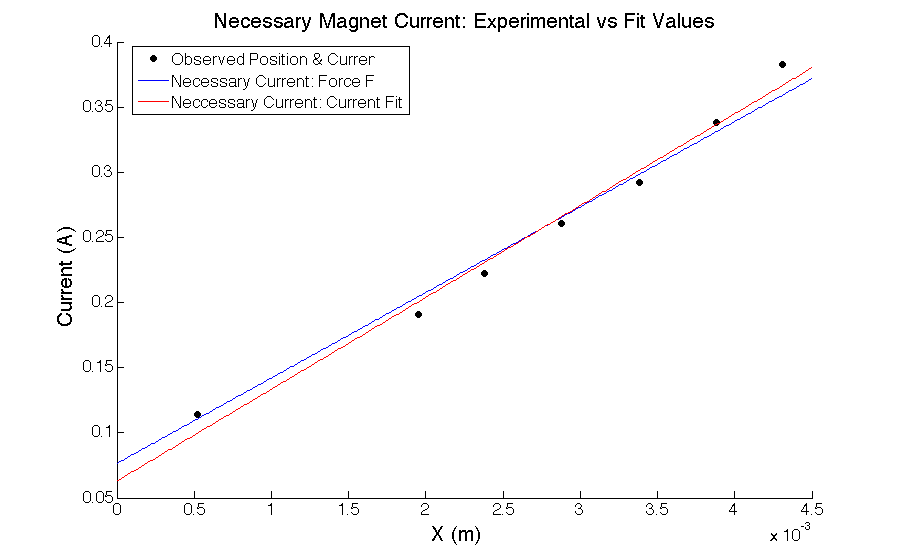
\includegraphics[width = 10cm]{magnetDataFits.png}
\end{center}
\label{Q1_d3}
\caption{Electromagnet Current vs X position}
\end{figure}

\begin{table}
\begin{center}
    \begin{tabular}{|c|c|c|c|}
        \hline
        ~           & A          & B         &  Error \\ \hline
        Force Fit   & 2.2795e-05 & 0.0011656  & 0.0223076 N \\ 
        Current Fit & 1.9752e-05 & 8.9294e-04 & 0.0272997 A\\
        \hline
    \end{tabular}
\end{center}
\caption{Two different parameter fits to our data}
\label{Q1_dt2}
\end{table}

\subsubsection*{Steel Sphere}
The steel sphere has two parameters of consequence for our modeling, its diameter and its mass.  Both of these values were obtained through direct measurements using calipers and a scale respectively.

\begin{table}[hbt]
\begin{center}
    \begin{tabular}{|c|c|}
        \hline
        Steel Sphere Mass (g)      & 10   \\ \hline
        Steel Sphere Diameter (mm) & 12.7 \\
        \hline
    \end{tabular}
\end{center}
\caption{Steel sphere parameters}
\label{Q1_dt3}
\end{table}


\subsection*{e.}

\subsection*{f.}

\subsection*{g.}

\section*{Part 2 Question 2}

\subsection*{a.}

\subsection*{b.}

\subsection*{c.}

\subsection*{d.}

\section*{Question 3}

\section*{Appendix}
\xxx{include radianceDerivative from part 1 folder}


\end{document}